\chapter{Desenvolvendo o primeiro projeto com o MDArte}

Neste capítulo iremos construir um projeto básico usando o MDArte. O projeto
consistirá de um sistema web simples para administrar um ambiente acadêmico,
onde poderemos cadastrar cursos e gerenciar suas informações, bem como inserir
alunos, inscrevê-los nos e gerenciar suas informações.

\section{Criação de um Novo Projeto}

O plugin do MDArte para o \texttt{Maven} já possui um procedimento parametrizado
para criação de projetos, que funciona como um \texttt{wizard}, onde o usuário
deve responder a perguntas. Através das respostas fornecidas, o MDArte
direcionará a criação da estrutura básica e dos artefatos básicos de
configuração de projetos. O procedimento para criação de um novo projeto é:

\begin{enumerate}
\item Abra o terminal (\texttt{command prompt}) e vá para o diretório onde se
deseja criar o projeto. O projeto será gerado em um subdiretório do
diretório escolhido com o mesmo nome da pasta definido na geração do projeto.

\item Digite o comando: \texttt{maven andromdapp:generate}

\item As perguntas devem ser respondidas de acordo com o projeto a ser
desenvolvido. Abaixo as respostas adequadas para o exemplo desenvolvido neste
capítulo (perguntas em negrito):

\textbf{Please enter your first and last name (i.e. Rodrigo Salvador):} \\
MDArte\\
\textbf{Please enter the name of your J2EE project (i.e. Sistema Academico):}\\
Sistema Academico\\
\textbf{Please enter the id for your J2EE project (i.e. sistemaacademico):}\\
sistemaacademico\\
\textbf{Please enter a version for your project (i.e. 1.0):}\\
1.0\\
\textbf{Please enter the base package name for your J2EE project (i.e. br.mdarte.exemplo.academico):}\\
br.mdarte.exemplo.academico\\
\textbf{Would you like to enable security? (enter 'yes' or 'no')?}\\
yes\\
\textbf{Would you like to use oAuth (enter 'yes' or 'no') ?}\\
no\\
\textbf{Would you like to use MDArte's default Controle Acesso (enter 'yes' or
'no') ?}\\
yes\\
\textbf{Would you like to use modules (enter 'yes' or 'no')?}\\
yes\\
\textbf{Please enter the EJB version number (enter '2' or '3'):}\\
3\\
\textbf{Please enter the Struts version number (enter '1' or '2'):}\\
2\\
\textbf{Would you like to enable the JUnit support for general testing? (enter
'yes' or 'no')? }\\
 no\\
\textbf{Please enter the database backend for the persistence layer: (enter
'hypersonic' or 'mysql' or 'oracle' or 'postgres')}\\
 postgres\\
 
\item Após receber as respostas, o MDArte criará um subdiretório onde será
gerada a estrutura inicial do projeto. A partir desse momento chamaremos esse
diretório de \texttt{<DiretorioProjeto>}.

\item Ainda no console, vá para o diretório onde está seu projeto:
\texttt{<DiretorioProjeto>}.

\item Digite \texttt{maven}. Isto obrigará o \texttt{Maven} a obter todos os
artefatos (por exemplo, bibliotecas) de que o projeto dependerá.

\end{enumerate}

\section{Controle de Acesso}

Neste tutorial estaremos utilizando funcionalidades de controle de acesso, porém
não é nosso propósito explorar suas funcionalidades. Assim, estaremos utilizando
um projeto de controle de acesso desenvolvido pela comunidade do MDArte.

O projeto pode ser obtido a partir do
\href{https://github.com/MDArte/controleacesso.git}{repositório} \texttt{Git} do
MDArte. Por fim, edite também o arquivo \texttt{project.properties} do
\texttt{ControleAcesso} para configurar o tipo de Banco de Dados a ser
utilziado, conforme realizado com o projeto SistemaAcademico. Note que a
propriedade \texttt{dataSource.name} está definida como
\texttt{controleacessoDS}.

Novamente, precisaremos criar um arquivo de configuração do Banco de Dados,
localizado no diretório
\texttt{\textdollar{}JBOSS\_HOME/server/default/deploy/}. O nome do arquivo deve
seguir a mesma formatação mencionada, terminando em \texttt{-ds.xml} (ex.:
\texttt{aplicacoes-ds.xml}), podendo estar no mesmo arquivo com as configurações
do projeto SistemaAcademico.

Exemplo:

\begin{framed}
	\lstinputlisting[language=xml]{files/ControleAcesso-ds.xml}
\end{framed}

Note que no exemplo anterior o ControleAcesso estará utilizando a mesma base de
dados do projeto SistemaAcademico, definida pela tag \texttt{<connection-url>}.
Agora, execute os seguinte comandos, na raiz do projeto \texttt{ControleAcesso},
para gerar, compilar e copiar os pacotes para o diretório
\texttt{\textdollar{}JBOSS\_HOMEHOME/server/default/deploy/}:

\begin{framed}
	\lstinputlisting[language=bash]{files/compila-ca}
\end{framed}

\section{Modelando o nosso primeiro projeto}

Vamos começar agora a modelar o nosso exemplo, mostrando o quão rápido e simples
pode ser usar o MDArte e todo o seu poder de geração.

Para esta parte do tutorial usaremos o \texttt{MagicDraw}. Na barra de
ferramentas do \texttt{MagicDraw}, clicaremos em \texttt{Open Project} e
abriremos o xml do projeto, \texttt{SistemaAcademico.xml} no caminho
\texttt{<DiretorioProjeto>/mda/src/uml/}.

\subsection{Modelando a camada de domínio}
Na camada de domínio, estarão as classes do domínio da aplicação. Elas serão
entidades e estarão associadas a algum modo de persistência. Afim de
contornar os problemas provenientes da utilização de bancos de dados relacionais
em conjunto com o paradigma de orientação à objeto, o MDArte usa o \texttt{framework}
\texttt{Hibernate}\footnote{\hypertarget{http://hibernate.org/orm/}{http://hibernate.org/orm/}}
para gerenciar esta camada.

As classes da camada de domínio deverão conter o estereótipo \texttt{«Entity»} e
os atributos que serão persistidos. Todas as classes de entidade serão
concentradas no pacote \texttt{<PacoteProjeto>.cd}, em que
\texttt{<PacoteProjeto>} é o pacote definido para o projeto. Note que não é
obrigatório que as classes da camada de domínio estejam todas no pacote
\texttt{<PacoteProjeto>.cd}, no entanto esta é uma boa prática e um padrão
adotado pela comunidade do MDArte.

Neste exemplo, especificamente, iremos também marcar nossas entidades com o
estereótipo \texttt{«Manageable»}, tal marcação diz para o MDArte que desejamos
que seja gerado um \texttt{CRUD\footnote{CRUD é um acrônimo de Create, Read,
Update e Delete em língua Inglesa para as quatro operações básicas utilizadas em
bancos de dados relacionais ou em interface para usuários para criação,
consulta, atualização e destruição de dados.}} padrão para tais entidades, sem a
necessidade de modelarmos o mesmo diretamente.

\begin{enumerate}
\item Crie a mesma estrutura de pacotes que foi definida na criação do projeto.
Dentro da estrutura, crie o pacote “cd”. Podemos ver o resultado na imagem
~\ref{cria_estrutura_pacotes}. 
\begin{figure}[H]
	\centering
	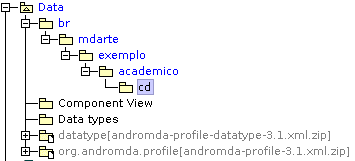
\includegraphics[width=250pt,height=100pt]{imgs/tutorial-mdarte-0000.png}
	\caption{Criação da estrutura de pacotes do projeto e do pacote cd.}
	\label{cria_estrutura_pacotes}
\end{figure}
\item Clique com o botão direito do mouse no pacote “cd” e selecione a opção
\texttt{New Diagram} .Em seguida, selecione \texttt{Class Diagram}. Como mostra
a Figura \ref{cria_diagrama_classe}.
\begin{figure}[H]
	\centering
	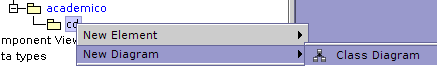
\includegraphics[width=400pt,height=60pt]{imgs/tutorial-mdarte-0001.png}
	\caption{Criação do diagrama de classes da camada de domínio.}
	\label{cria_diagrama_classe}
\end{figure}
	
\item Indique o nome desejado para o diagrama (ex: Entidades).
	
\item No diagrama de classe, crie uma nova classe. Clique com o botão direto
sobre a classe e selecione a opção \texttt{Specification}. Defina o nome da
classe como \texttt{“Estudante”}.
	
\item Crie os atributos na classe Estudante (matricula, nome) selecionando a aba
\texttt{Attributes} e clicando no botão \texttt{Add}. A figura abaixo
exemplifica a criação do atributo matricula. O campo \texttt{Visibility} deve
ser \texttt{public}. Não é necessário modelar o atributo \texttt{id}, pois ele é
gerado automaticamente. Como mostra a Figura \ref{config_parametro}.

\begin{figure}[H]
	\centering
	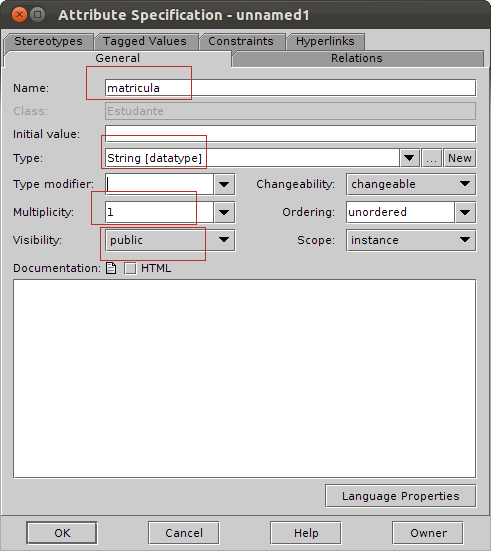
\includegraphics[width=350pt,height=400pt]{imgs/tutorial-mdarte-0002.png}
	\caption{Configuração do parâmetro matrícula da classe Estudante.}
	\label{config_parametro}
\end{figure}
		
A multiplicidade com valor 1 (campo \texttt{Multiplicity}) indica que o atributo é
obrigatório (\texttt{NOT NULL} ), já o valor \texttt{0..1} indica que o atributo
não é obrigatório. Por padrão, todos os atributos são gerados como \texttt{NOT
NULL}.

\item Coloque o estereótipo \texttt{«Unique»} no atributo \texttt{matricula}
para indicar que cada código deve ser único, ou seja, não pode haver duas
matrículas iguais. Abra a especificação do atributo \texttt{matricula} e
selecione a aba \texttt{Stereotypes}. Nessa aba selecione o estereótipo
\texttt{«Unique»}, como na figura \ref{add_estereotipo_matricula}.

\begin{figure}[H]
	\centering
	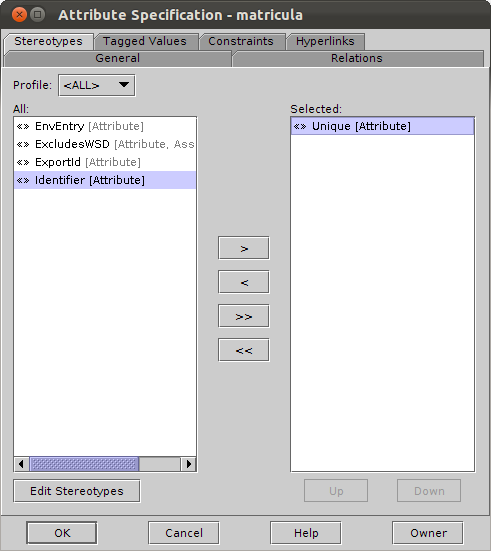
\includegraphics[width=350pt,height=400pt]{imgs/tutorial-mdarte-0003.png}
	\caption{Adição de estereótipo no atributo matrícula.}
	\label{add_estereotipo_matricula}
\end{figure}
	
\item Coloque os estereótipos \texttt{«Entity»} e \texttt{«Manageable»} na
classe \texttt{Estudante}, como na figura \ref{add_estereotipo_estudante}. 
\begin{figure}[H]
	\centering
	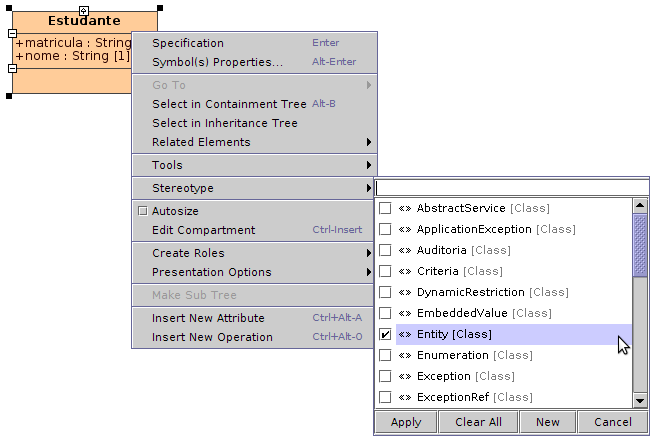
\includegraphics[width=400pt,height=300pt]{imgs/tutorial-mdarte-0004.png}
	\caption{Adição dos estereótipos Entity e Manageable na classe estudante.}
	\label{add_estereotipo_estudante}
\end{figure}
	
\item No mesmo diagrama de classes, crie outra classe. Clique com o botão direto
sobre a classe e selecione a opção \texttt{Specification}. Defina o nome da classe como
\texttt{“Curso”}.
	
\item Crie os atributos na classe \texttt{Curso} (\texttt{codigo},
\texttt{nome}) selecionando a aba \texttt{Attributes} e clicando no botão
\texttt{Add}. O campo \texttt{Visibility} deve ser \texttt{public}, assim como
feito anteriormente.

\item Coloque o estereótipo \texttt{«Unique»} no atributo codigo para indicar
que cada código deve ser único. Abra a especificação do atributo codigo e
selecione a aba \texttt{Stereotypes}. Nessa aba selecione o estereótipo
\texttt{«Unique»}.
	
\item Coloque o estereótipo \texttt{«Entity»} na classe.
	
\item Agora, crie uma associação entre as classes. Vá no diagrama de classes e
puxe uma relação \texttt{Association} de uma classe para outra.
	
\item A associação será de \texttt{1 para muitos}. Assim, clique duas vezes na associação
e irá aparecer a tela de especificação. Edite os campos \texttt{Multiplicity} definindo
valor “0..*” para a entidade \texttt{Estudante} e “1” para a entidade
\texttt{Curso}, como na figura ~\ref{define_multiplicidade_associacao}.
\begin{figure}[H]
	\centering
	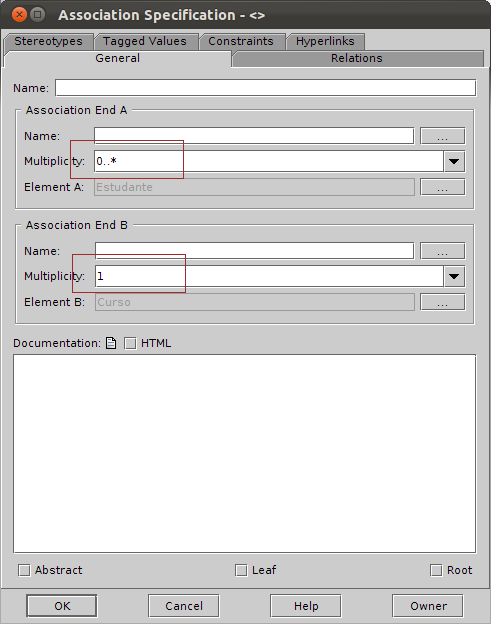
\includegraphics[width=350pt,height=400pt]{imgs/tutorial-mdarte-0005.png}
	\caption{Definindo multiplicidade da associação.}
	\label{define_multiplicidade_associacao}
\end{figure}
	
\item A associação deve ser dupla, tanto \texttt{Estudant} e quanto
\texttt{Curso} devem ser visíveis. Dessa forma, mantenha a \texttt{checkbox}
\texttt{Navigable} marcada na associação para as duas classes. Para isso, clique
no botão “...” (reticências) da tela anterior, como na imagem
~\ref{config_navigable_associacao}.
\begin{figure}[H]
	\centering
	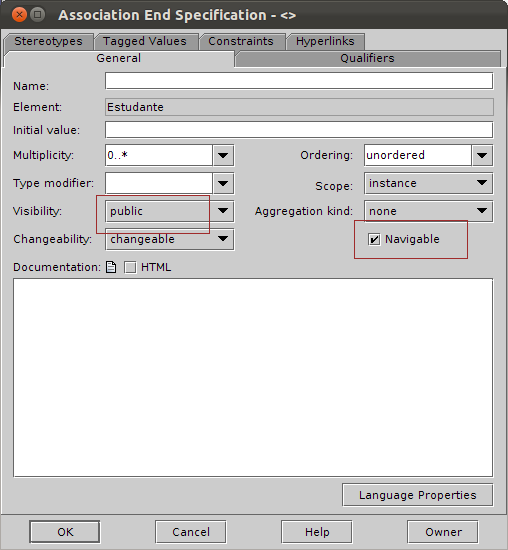
\includegraphics[width=350pt,height=400pt]{imgs/tutorial-mdarte-0006.png}
	\caption{Configuração da navegabilidade da associação.}
	\label{config_navigable_associacao}
\end{figure}
		
O resultado final pode ser visto na imagem ~\ref{resultado_diagrama_classe}: \hfill

\begin{figure}[H]
	\centering
	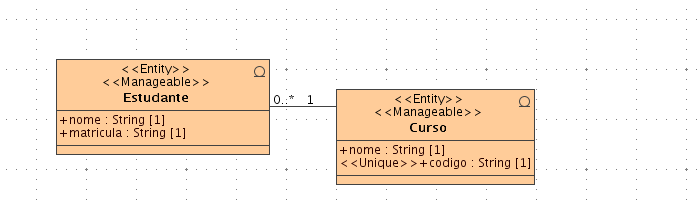
\includegraphics[width=500pt,height=200pt]{imgs/tutorial-mdarte-0007.png}
	\caption{Resultado final da modelagem da camada de domínio.}
	\label{resultado_diagrama_classe}
\end{figure}
	
\item No diretório da aplicação, execute o comando maven para validar o modelo e
gerar o script \texttt{SQL} de criação do Banco de Dados. O resultado
apresentado deve ser \texttt{“BUILD SUCCESFULL”}.
	
\item Observe que dois novos arquivos \texttt{xml} terão sido criados no caminho
\texttt{<DiretorioProjeto>/mda/src/uml/} com os nomes
\texttt{sistemaacademico-geral-Curso.xml} e
\texttt{sistemaacademico-geral-Estudante.xml} , com os
\texttt{CRUD} \texttt{default} gerados pelo MDArte. Agora precisamos importar os
casos de uso criados pelo MDArte para o \texttt{xml} geral do nosso projeto
(\texttt{SistemaAcademico.xml}). Para isso iremos na barra de ferramentas do
\texttt{MagicDraw} clicaremos em \texttt{file} e na lista de opções que se
abrirá clicaremos em \texttt{import}. Na janela que se abrirá selecionaremos os
modelos que queremos adicionar e clicaremos em \texttt{open}, como na imagem
~\ref{importa_modulo_geral}:
 \begin{figure}[H]
	\centering
	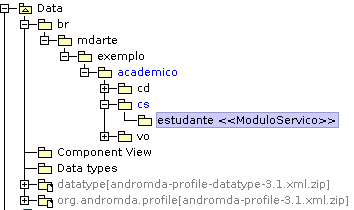
\includegraphics[width=240pt,height=200pt]{imgs/tutorial-mdarte-0008.png}
	\caption{Criação do pacote para a camada de serviço.}
	\label{importa_modulo_geral}
\end{figure} 

O resultado da importação na nossa estrutura de diretórios pode ser visto na
imagem \ref{resultado_arvore_diretórios}.
\begin{figure}[H]
	\centering
	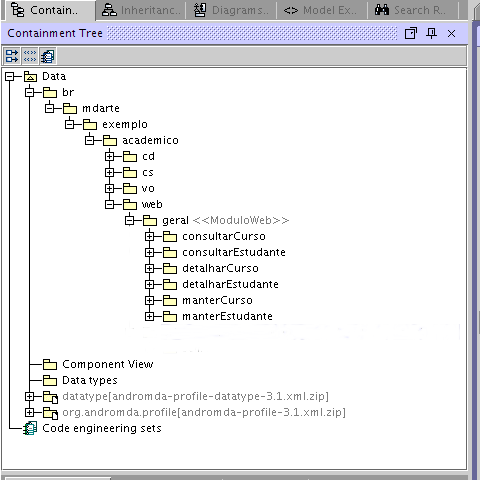
\includegraphics[width=300pt,height=300pt]{imgs/tutorial-mdarte-0019.png}
	\caption{Arvore de diretórios do projeto após a importação dos CRUD gerados
	automaticamente.}
	\label{resultado_arvore_diretórios}
\end{figure} 

Agora precisamos regerar o projeto, bem como os módulos separados, para isso,
executaremos então os comandos:
	
\begin{framed}
	\lstinputlisting[language=bash]{files/compila-cruds}
\end{framed}

\end{enumerate}

\textbf{* Ao fim dessa seção falar com o Glauco ou o Felipe Milepe sobre o
modelo de CRUD gerado automaticamente.}

\subsection{Criando o Banco de Dados}

Durante a execução do comando \texttt{maven}, todas as classes são criadas
automaticamente. Além disso, também é gerado o código \texttt{SQL} de criação de
tabelas do Banco de Dados. O script \texttt{SQL} pode ser encontrado em
\texttt{<DiretorioProjeto>/core/cd/target/schema-create.sql}. Abrindo o arquivo
é possível notar a presença de comandos de crição das tabelas \texttt{ESTUDANTE}
e \texttt{CURSO}.

Execute o conteúdo do arquivo no Banco de Dados utilizado.

Como exemplificação dos casos de usos que serão elaborados por este documento,
execute o seguinte script \texttt{SQL} para criar a base inicial. Note que o
script foi escrito para PostgreSQL e deve ser adaptado para o Banco de Dados
escolhido.

\begin{framed}
	\lstinputlisting[language=sql]{files/exemplo.sql}
\end{framed}

\subsection{Modelando a camada de serviços}

Na camada de serviço serão implementadas as classes responsáveis pela lógica de
negócio da aplicação. As classes especificadas se tornarão os serviços
(\texttt{API}) da aplicação. Os serviços definidos no modelo se tornarão
disponíveis através de \texttt{Session Beans}.

Os \texttt{Session Beans} são componentes de negócio. A lógica de negócio dos
componentes \texttt{EJB} se encontram nestes componentes. Existem dois tipos de
Componentes \texttt{Session Bean}, o \texttt{Stateless Session Bean} e o
\texttt{Stateful Session Beans}. O \texttt{Stateless} é um componente de negócio
que não mantém conversação com o usuário, não há garantia que chamadas
sucessivas de métodos remotos vão ser feitas no mesmo objeto. O
\texttt{Stateful} é um componente que mantêm estado, com ele temos a garantia
que chamadas sucessivas de métodos remotos feitas por um mesmo cliente serão
processadas por um mesmo objeto.

Os \texttt{beans} \texttt{EJB} precisam ser modelados em um diagrama de classes.
As classes destes beans precisam ter o estereótipo \texttt{«Service»}. Todas as
classes de serviço devem estar no pacote \texttt{<PacoteProjeto>.cs}, em que
\texttt{<PacoteProjeto>} é o pacote definido para o projeto.

\begin{enumerate}
\item Crie um pacote \texttt{<PacoteProjeto>.cs.estudante}. Clique então com o
botão direito sobre a pasta estudante, na opção \texttt{Stereotype}, selecione o
estereótipo \texttt{«ModuloServico»} e clique em \texttt{Apply}. O resultado
pode ser visto na imagem ~\ref{cria_pacote_servico}:
 \begin{figure}[H]
	\centering
	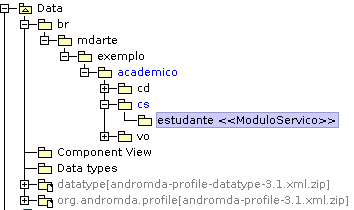
\includegraphics[width=240pt,height=200pt]{imgs/tutorial-mdarte-0008.png}
	\caption{Criação do pacote para a camada de serviço.}
	\label{cria_pacote_servico}
\end{figure} 
	
\item Crie um diagrama de classe dentro do pacote \texttt{estudante}, com o nome
que desejar.
	
\item Crie uma classe com nome \texttt{EstudanteHandler} e estereótipo
\texttt{«Service»}.A classe \texttt{EstudanteHandler} deve ficar como na figura
\ref{cria_sevico_estudante}.
\begin{figure}[H]
	\centering
	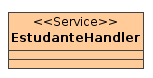
\includegraphics[width=150pt,height=120pt]{imgs/tutorial-mdarte-0009.png}
	\caption{Criação da classe de serviço EstudanteHandler.}
	\label{cria_sevico_estudante}
\end{figure} 
	
\item Crie uma classe com nome \texttt{EstudanteException} e estereótipo
\texttt{«ApplicationException»}, como na imagem ~\ref{cria_estudante_exception}.
\begin{figure}[H]
	\centering
	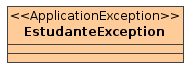
\includegraphics[width=150pt,height=120pt]{imgs/tutorial-mdarte-0010.png}
	\caption{Criação da classe estudante exception.}
	\label{cria_estudante_exception}
\end{figure}
	
\item Arraste para o diagrama de classes recém criado no pacote estudante a
classe \texttt{Estudante}.
	
\item Crie uma relação de dependência entre as classes \texttt{EstudanteHandler}
e \texttt{Estudante}, assim como entre \texttt{EstudanteHandler} e
\texttt{EstudanteException}. Para isso, utilize a opção do \texttt{MagicDraw}
ilustrada na figura abaixo. Clique na opção, depois clique na classe, ou método,
de origem e arraste a seta até a classe destino, como na imagem
\ref{cria_dependencia_servico}.

\begin{figure}[H]
	\centering
	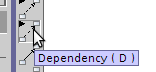
\includegraphics[width=110pt,height=90pt]{imgs/tutorial-mdarte-0012.png}
	\caption{Criação da dependência entre as classes do serviço.}
	\label{cria_dependencia_servico}
\end{figure}

\item Verifique se o diagrama está como a figura
\ref{resultado_diagrama_classe_servico}.
\begin{figure}[H]
	\centering
	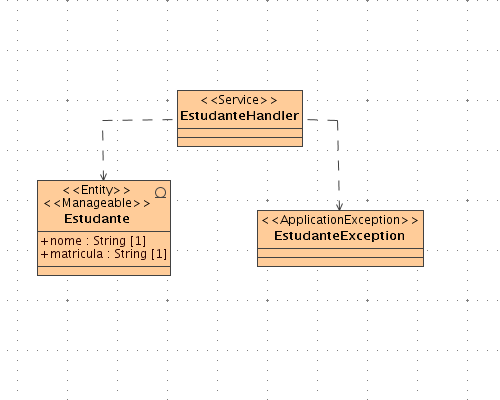
\includegraphics[width=360pt,height=350pt]{imgs/tutorial-mdarte-0011.png}
	\caption{Diagrama de classe completo do módulo de serviço para a classe
	Estudante.}
	\label{resultado_diagrama_classe_servico}
\end{figure}

\item A dependência entre \texttt{EstudanteHandler} e
\texttt{EstudanteException} fará com que todos os métodos de
\texttt{EstudanteHandler} possam lançar a exceção \texttt{EstudanteException}.
Se a dependência tivesse sido entre algum método de \texttt{EstudanteHandler} e
não com a própria classe, somente o método com dependência poderia lançar a
exceção.

A dependência entre \texttt{EstudanteHandler} e \texttt{Estudante} cria os
métodos de acesso ao banco na classe de serviço.

\item Agora faça o mesmo para criar um modulo de serviço para a classe
\texttt{Curso}.
	
\item No diretório da aplicação, execute o comando maven para validar o modelo e
gerar as classes de serviço. O resultado apresentado deve ser \texttt{“BUILD
SUCCESSFULL”}.
\end{enumerate}

\section{Implementando as classes de controle dos \texttt{CRUD} gerados}

Nessa seção vamos implementar as classes de controle dos casos de uso gerados.
Para isso, abriremos os arquivos \texttt{<nomeCasoDeUso>ControleImpl}.java.
Esses arquivos são pontos de implementação onde deve ser concentrado todo o
código que se queira adicionar manualmente às classes de controle. Como tais
arquivos só são gerados caso ainda não existam, o código colocado neles não será
sobrescrito, ao contrario do que ocorre se inserirmos manualmente codigo nos
arquivos \texttt{<nomeCasoDeUso>Controle.java}.

De acordo com os casos de uso gerados automaticamente pelo gerador de
\texttt{CRUD} do MDArte, iremos implementar respectivamente os seguintes código
nos seguintes arquivos, que devem portanto ser abertos no \texttt{Eclipse} ou em
outra \texttt{IDE} desejada:

\begin{enumerate}
\item ConsultaEstudanteControleImpl.java :
\begin{framed}
	\lstinputlisting[language=java]{files/ConsultaEstudanteControleImpl.java}
\end{framed}
		
\item MantemEstudanteControleImpl.java :
\begin{framed}
	\lstinputlisting[language=java]{files/MantemEstudanteControleImpl.java}
\end{framed}

\item DetalhaEstudanteControleImpl.java:
\begin{framed}
	\lstinputlisting[language=java]{files/DetalhaEstudanteControleImpl.java}
\end{framed}

\item ConsultaCursoControleImpl.java :
\begin{framed}
	\lstinputlisting[language=java]{files/ConsultaCursoControleImpl.java}
\end{framed}

\item MantemCursoControleImpl.java :
\begin{framed}
	\lstinputlisting[language=java]{files/MantemCursoControleImpl.java}
\end{framed}

\item DetalhaCursoControleImpl.java :
\begin{framed}
	\lstinputlisting[language=java]{files/DetalhaCursoControleImpl.java}
\end{framed}

\end{enumerate}

Agora, no terminal, no <DiretorioProjeto> executaremos o seguinte comando :

\begin{framed}
	\lstinputlisting[language=bash]{files/compile-deploy}
\end{framed}

\subsection{Inicializando o servidor e testanto a aplicação}

O \texttt{eclipse} nos fornece a possibilidade de fazer o gerenciamento do
servidor \texttt{JBoss} dentro da própria IDE. Para isso precisamos criar, na
IDE, um novo servidor. 

Primeiramente, certifique-se de que você está usando a perspectiva de
desenvolvimento \texttt{Java EE}. No conjunto de abas na parte
inferior da IDE, abaixo da parte onde fica o código, selecione a aba
\texttt{servers} como na imagem \ref{seleciona_server_eclipse} .

\begin{figure}[H]
	\centering
	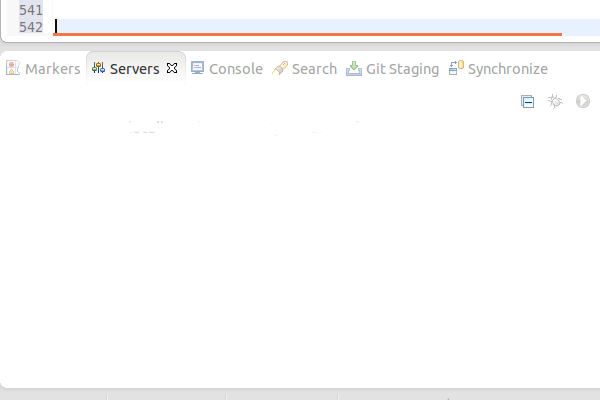
\includegraphics[width=400pt,height=250pt]{imgs/tutorial-mdarte-0021.png}
	\caption{Inicializando o servidor JBoss.}
	\label{seleciona_server_eclipse}
\end{figure}

Agora clique com o botão direito no espaço vazio, vá em \texttt{new > server}.
Será aberta a janela \texttt{'New Server'}. Preencha os dados como na imagem
\ref{cria_server_eclipse}.

\begin{figure}[H]
	\centering
	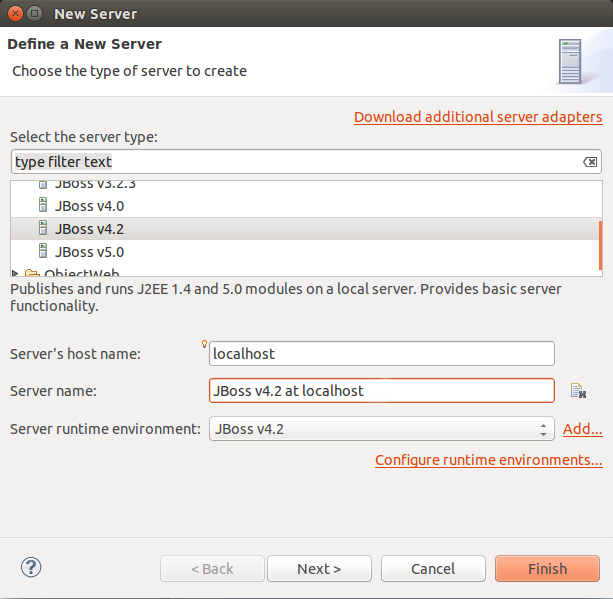
\includegraphics[width=400pt,height=320pt]{imgs/tutorial-mdarte-0022.png}
	\caption{Inicializando o servidor JBoss.}
	\label{cria_server_eclipse}
\end{figure}

Agora daremos \texttt{Start} no servidor \texttt{Jboss} e verificaremos então no
navegador o resultado do nosso sistema. Para dar \texttt{Start} no servidor
iremos na aba \texttt{Servers} no nossa \texttt{IDE}, selecionaremos o servidor
e clicaremos então no botão de \texttt{Start} (Verde), como na imagem
\ref{server_start}:
\begin{figure}[H]
	\centering
	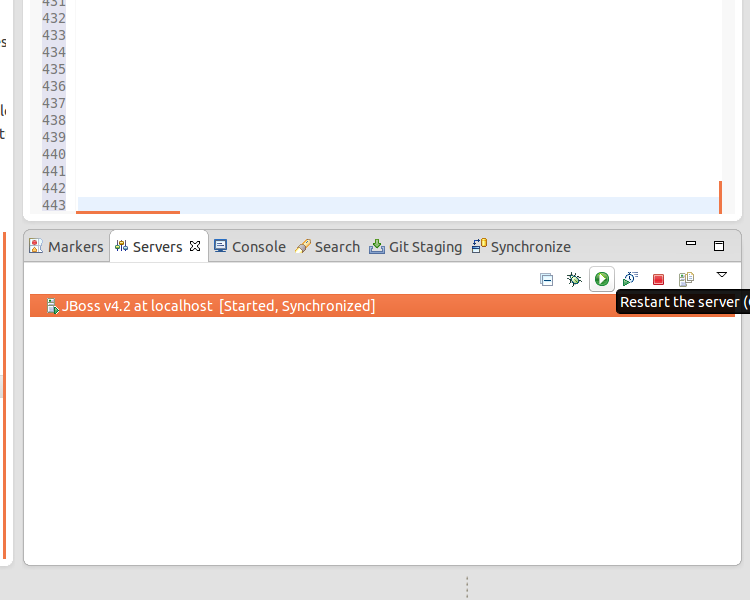
\includegraphics[width=400pt,height=250pt]{imgs/tutorial-mdarte-0015.png}
	\caption{Inicializando o servidor JBoss.}
	\label{server_start}
\end{figure}

Para acessar o sistema, abriremos o navegador e acessaremos a url
\texttt{http://localhost:8080/sistemaacademico/}. Primeiramente será aberta a
página de login do sistema, como na imagem \ref{pagina_login}:
\begin{figure}[H]
	\centering
	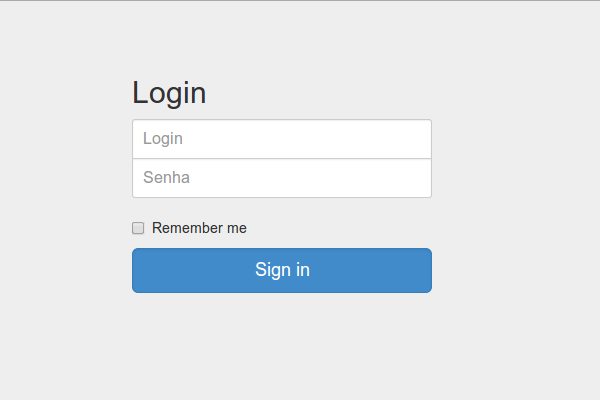
\includegraphics[width=300pt,height=250pt]{imgs/tutorial-mdarte-0013.png}
	\caption{Página de login do Sistema Acadêmico.}
	\label{pagina_login}
\end{figure}

Feito o login, a tela inicial do sistema será aberta como na imagem
\ref{pagina_inicial}.
\begin{figure}[H]
	\centering
	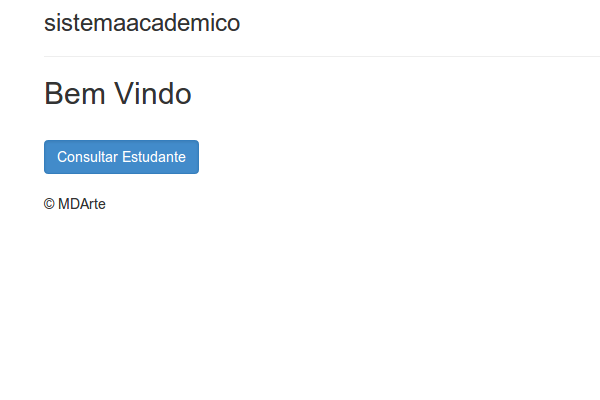
\includegraphics[width=400pt,height=320pt]{imgs/tutorial-mdarte-0017.png}
	\caption{Página incial do Sistema Acadêmico.}
	\label{pagina_inicial}
\end{figure}

Ao clicar no botão \texttt{Consulta Estudante} seremos redirecionados para a
página de consulta no caso de uso de mesmo nome como na imagem
\ref{pagina_consulta_estudante}.
\begin{figure}[H]
	\centering
	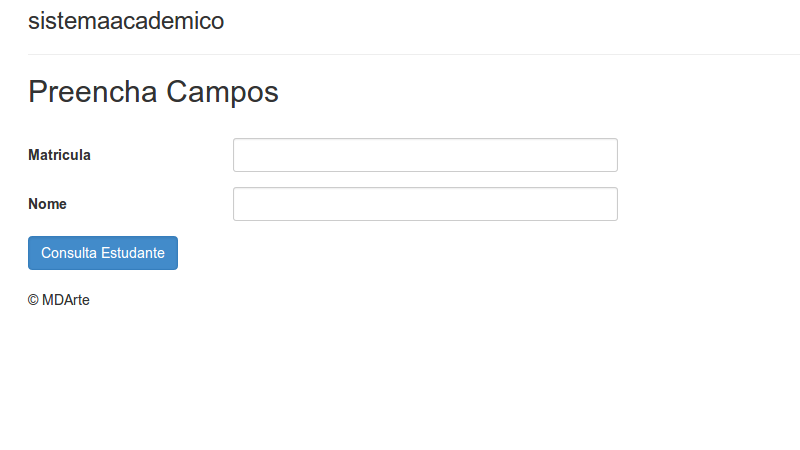
\includegraphics[width=400pt,height=320pt]{imgs/tutorial-mdarte-0018.png}
	\caption{Página incial de Consulta Estudante.}
	\label{pagina_consulta_estudante}
\end{figure}

Se pesquisarmos sem nenhum filtro veremos uma lista completa dos estudantes
registrados como na imagem \ref{resultado_busca_sem_filtro}.
\begin{figure}[H]
	\centering
	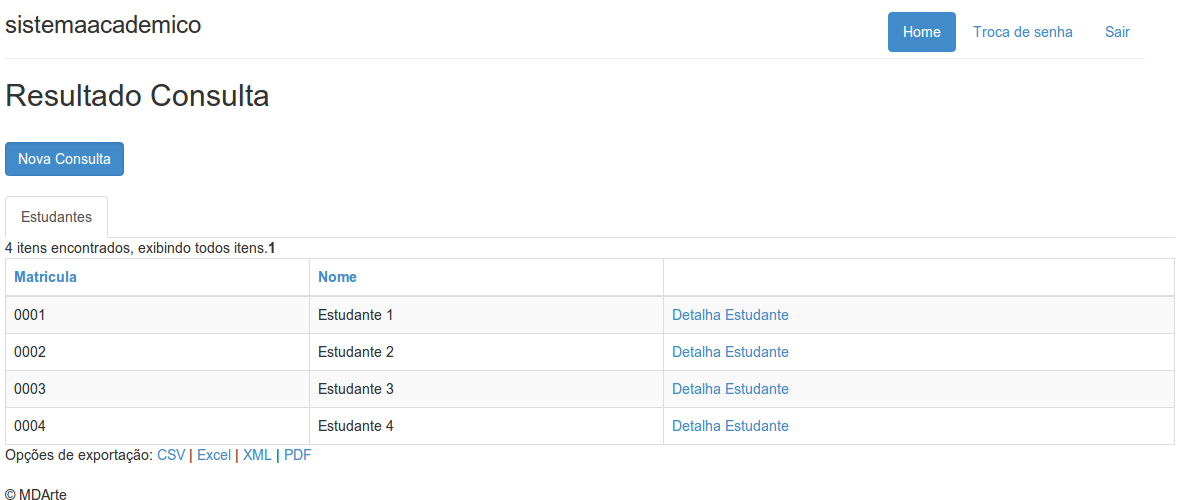
\includegraphics[width=500pt,height=320pt]{imgs/tutorial-mdarte-0020.png}
	\caption{Resultado da busca sem filtro pelos estudantes.}
	\label{resultado_busca_sem_filtro}
\end{figure}










